\chapter{\ifproject%
\ifcpe โครงสร้างและขั้นตอนการทำงาน\else Project Structure and Methodology\fi
\else%
\ifcpe โครงสร้างของโครงงาน\else Project Structure\fi
\fi
}


\makeatletter

% \renewcommand\section{\@startsection {section}{1}{\z@}%
%                                    {13.5ex \@plus -1ex \@minus -.2ex}%
%                                    {2.3ex \@plus.2ex}%
%                                    {\normalfont\large\bfseries}}

\makeatother
%\vspace{2ex}
% \titleformat{\section}{\normalfont\bfseries}{\thesection}{1em}{}
% \titlespacing*{\section}{0pt}{10ex}{0pt}
ในบทนี้จะกล่าวถึงผลสรุปจากการสํารวจความคิดเห็นของนักศึกษาเกี่ยวกับตารางสอบปลายภาค ข้อมูลที่จำเป็นต้องใช้สำหรับการพัฒนาโปรแกรม รวมถึงโครงสร้างข้อมูลรับเข้าและข้อมูลส่งออกของโปรแกรม
ซึ่งจากความต้องการพัฒนาระบบจัดตารางสอบปลายภาคเพื่อให้นักศึกษามีอิสระในการเลือกลงทะเบียนเรียนมากขึ้นดังที่กล่าวในตอนที่ \ref{sec:project_rationale} เราจึงต้องการทราบความคิดเห็นของนักศึกษาในมหาวิทยาลัยเชียงใหม่เกี่ยวกับตารางสอบปลายภาค 
ทำให้เราได้จัดทำแบบสอบถามขึ้นเพื่อสอบถามความคิดเห็นของนักศึกษามหาวิทยาลัยเชียงใหม่ ทั้งนักศึกษาปัจจุบันและนักศึกษาที่สำเร็จการศึกษาแล้ว ว่ามีความคิดเห็นอย่างไรกับตารางสอบปลายภาคในปัจจุบัน และหากเลือกได้อยากจะสอบในช่วงเวลาใดบ้าง ๆ ในตารางเวลาของสัปดาห์ที่จัดสอบ 
โดยจะพยายามนำข้อมูลที่ได้มาใช้ในการอ้างอิงเพื่อออกแบบอัลกอริทึมสำหรับประมวลผลหาวิธีการจัดตารางสอบที่เหมาะสมที่สุดที่เป็นไปได้สำหรับนักศึกษาทุกคน

\section{การเก็บข้อมูล}
\subsection{การสำรวจความคิดเห็นของนักศึกษาเกี่ยวกับตารางสอบปลายภาค}
\CIreply{เพิ่มรายละเอียดว่าผู้ตอบแบบสอบถามมาจากคณะใดบ้าง ชั้นปี ฯลฯ}
\TSNAreply{เพิ่มละครับ}
จากผลสำรวจของแบบสอบถามเกี่ยวกับตารางสอบปลายภาคของมหาวิทยาลัยชียงใหม่ โดยขอความร่วมมือนักศึกษาในมหาวิทยาลัย
ทั้งนักศึกษาที่กำลังศึกษาอยู่และทั้งที่สำเร็จการศึกษาไปแล้ว เพื่อให้ช่วยตอบแบบสอบถามความคิดเห็นเกี่ยวกับ ข้อดี ข้อเสีย ความพึงพอใจในตารางสอบของตนเอง
รวมถึงปัญหาเกี่ยวกับตารางสอบปลายภาคที่เคยพบหรือได้รับผลกระทบโดยตรง โดยจากผลการสำรวจกลุ่มสำรวจจำนวน 95 คน สามารถแบ่งผู้ตอบแบบสอบถามตามระดับการศึกษาได้ 5 ระดับดังกราฟที่ \ref{fig:academic_year} โดยมีจำนวนดังนี้
\begin{itemize}
  \item ชั้นปีที่ 1 จำนวน 14 คน
  \item ชั้นปีที่ 2 จำนวน 27 คน
  \item ชั้นปีที่ 3 จำนวน 11 คน
  \item ชั้นปีที่ 4 จำนวน 38 คน
  \item มากกว่าชั้นปีที่ 4 จำนวน 2 คน
  \item สำเร็จการศึกษาแล้ว จำนวน 3 คน
\end{itemize}
\begin{figure}
  \begin{center}
    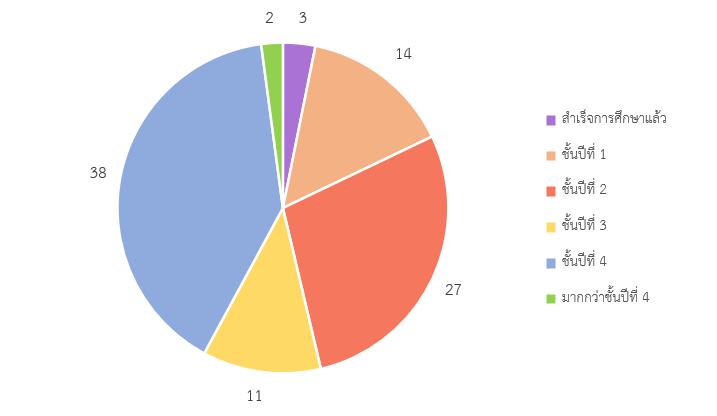
\includegraphics[width=\linewidth]{images/group_by_academic_year.png}
  \end{center}
  \caption[จำนวนผู้ตอบแบบสอบถามแบ่งตามชั้นปีที่ศึกษา]{จำนวนผู้ตอบแบบสอบถามแบ่งตามชั้นปีที่ศึกษา}
  \label{fig:academic_year}     
\end{figure}
และหากแบ่งผู้ตอบแบบสอบถามตามคณะที่ศึกษาจะสามารถแบ่งได้ดังกราฟที่ \ref{fig:faculty} 
โดยคณะอื่น ๆ ประกอบไปด้วยนักศึกษาจากคณะต่าง ๆ ดังนี้
\begin{itemize}
  \item คณะสังคมศาสตร์ จำนวน 2 คน
  \item คณะเกษตรศาสตร์ จำนวน 2 คน
  \item คณะเภสัชศาสตร์ จำนวน 1 คน
  \item คณะเทคนิคการแพทย์ จำนวน 2 คน
  \item คณะพยาบาลศาสตร์ จำนวน 1 คน
  \item คณะสัตวแพทยศาสตร์ จำนวน 2 คน
  \item คณะรัฐศาสตร์และรัฐประศาสนศาสตร์ จำนวน 1 คน
  \item วิทยาลัยศิลปะ สื่อ และเทคโนโลยี จำนวน 1 คน
\end{itemize}
\begin{figure}
  \begin{center}
    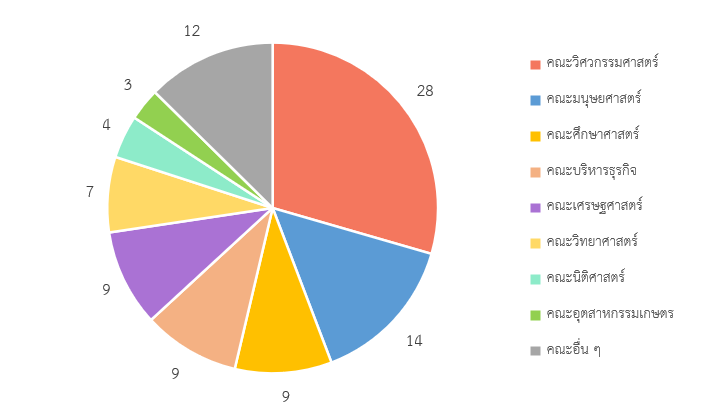
\includegraphics[width=\linewidth]{images/group_by_faculty.png}
  \end{center}
  \caption[จำนวนผู้ตอบแบบสอบถามแบ่งตามคณะที่ศึกษา]{จำนวนผู้ตอบแบบสอบถามแบ่งตามคณะที่ศึกษา}
  \label{fig:faculty}     
\end{figure}

โดยจากการสรุปผลการสำรวจพบว่าผู้ตอบแบบสอบถามส่วนใหญ่นั้นตรวจสอบตารางสอบของทุกวิชาที่ต้องการจะลงทะเบียน
ก่อนที่จะลงทะเบียนเรียนอย่างสม่ำเสมอ แต่ยังมีผู้ตอบแบบสอบถามบางส่วนนั้นที่ตรวจสอบตารางสอบเพียงบางวิชาก่อนจะลงทะเบียนเรียน และยังมีมีผู้ตอบแบบสอบถามส่วนน้อยที่ตอบว่าไม่เคยตรวจสอบตารางสอบของตนเองเลย ดังกราฟที่ \ref{fig:check_before_enrollment}
\begin{figure}
  \begin{center}
    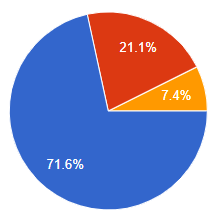
\includegraphics{images/checking_schedule_before_enrollment.png}\\[2ex]
    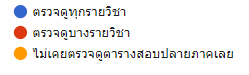
\includegraphics{images/legend_for_checking_schedule_before_enrollment.png}
  \end{center}
  \caption[จำนวนผู้ตอบแบบสอบถามที่ตรวจสอบตารางสอบปลายภาคก่อนการลงทะเบียน]{จำนวนผู้ตอบแบบสอบถามที่ตรวจสอบตารางสอบปลายภาคก่อนการลงทะเบียน}
  \label{fig:check_before_enrollment}     
\end{figure}
จากผลการสำรวจเรายังพบว่ากลุ่มสำรวจกว่า 80\% ไม่ทราบว่าสำนักทะเบียนมหาลัยเชียงใหม่ จัดตารางสอบปลายภาคอย่างไร ดังแสดงในกราฟที่ \ref{fig:registration_exam}
\begin{figure}
  \begin{center}
    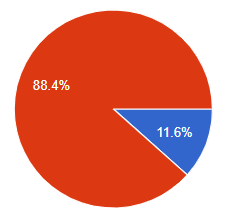
\includegraphics{images/registration_exam.png}\\[2ex]
    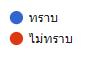
\includegraphics{images/legend_for_registration_exam.png}
  \end{center}
  \caption[จำนวนผู้ตอบแบบสอบถามที่ทราบวิธีการจัดตารางสอบปลายภาคของสำนักทะเบียน]{จำนวนผู้ตอบแบบสอบถามที่ทราบวิธีการจัดตารางสอบปลายภาคของสำนักทะเบียน}
  \label{fig:registration_exam}     
\end{figure}
จากผลการสำรวจเรายังสามารถสรุปผลได้ดังนี้
วันที่ผู้ทำแบบสอบถามต้องการจะสอบมากที่สุด 7 อันดับแรก โดยเรียงลำดับจากมากไปน้อย
\begin{enumerate}
  \item สัปดาห์ที่หนึ่ง วันจันทร์
  \item สัปดาห์ที่หนึ่ง วันพุธ
  \item สัปดาห์ที่หนึ่ง วันศุกร์ 
  \item สัปดาห์ที่หนึ่ง วันอาทิตย์
  \item สัปดาห์ที่สอง วันอังคาร
  \item สัปดาห์ที่สอง วันพฤหัสบดี
  \item สัปดาห์ที่สอง วันเสาร์
\end{enumerate}

จากข้อมูลเราสามารถบอกได้ว่าเวลาที่ผู้ทำแบบสอบถามส่วนใหญ่ต้องการที่จะสอบในแต่ละวันคือ
ช่วงเวลา 12.00-15.00น. ซึ่งผู้ทำแบบสอบถามส่วนมากต้องการจะสอบช่วงเวลานี้มากกว่า 15.30-18.00น. และ 08.00-11.00น. ตามลำดับ ดังกราฟ \ref{fig:time}
\begin{figure}
  \begin{center}
    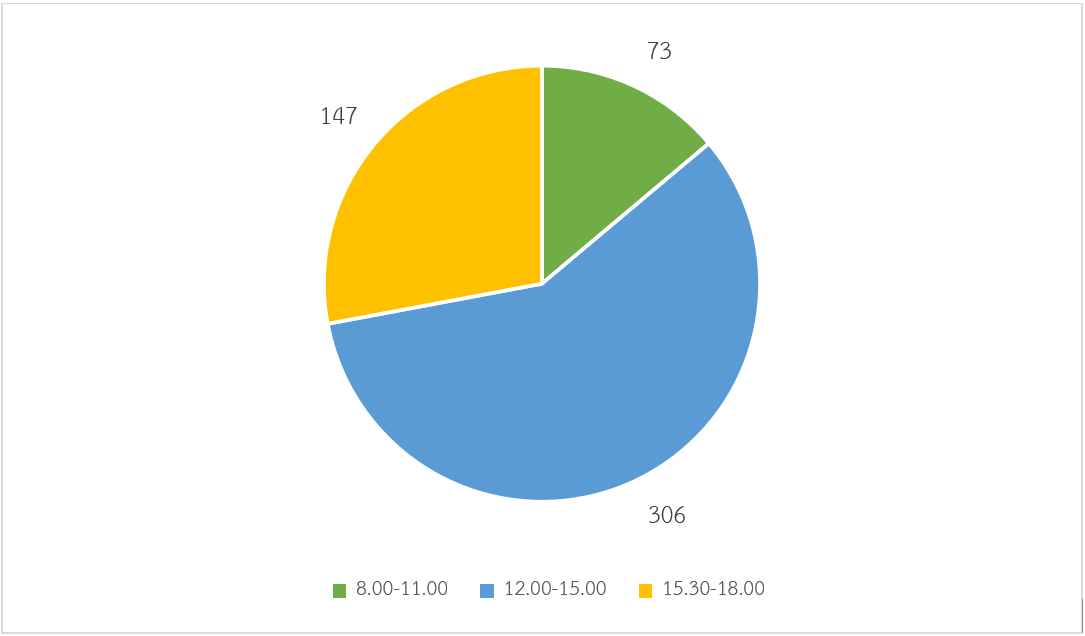
\includegraphics[width=\linewidth]{images/pie_chart_for_final_exam_time.png}
  \end{center}
  \caption[วามต้องการในการสอบของผู้ตอบแบบสอบถามในแต่ละเวลา]{ความต้องการในการสอบของผู้ตอบแบบสอบถามในแต่ละเวลา}
  \label{fig:time}
\end{figure}
และถ้าเราทำการรวมช่วงเวลาที่ผู้ตอบแบบสอบถามต้องการสอบกับวันที่ผู้ตอบแบบสอบถามต้องการสอบเข้าด้วยกันดังกราฟที่ \ref{fig:time_slot} จะสามารถสรุปวันที่ผู้ทำแบบสอบถามต้องการจะสอบมากที่สุด 7 อันดับแรก โดยสามารถเรียงลำดับจากมากไปน้อยได้ ดังนี้
\begin{figure}
  \begin{center}
    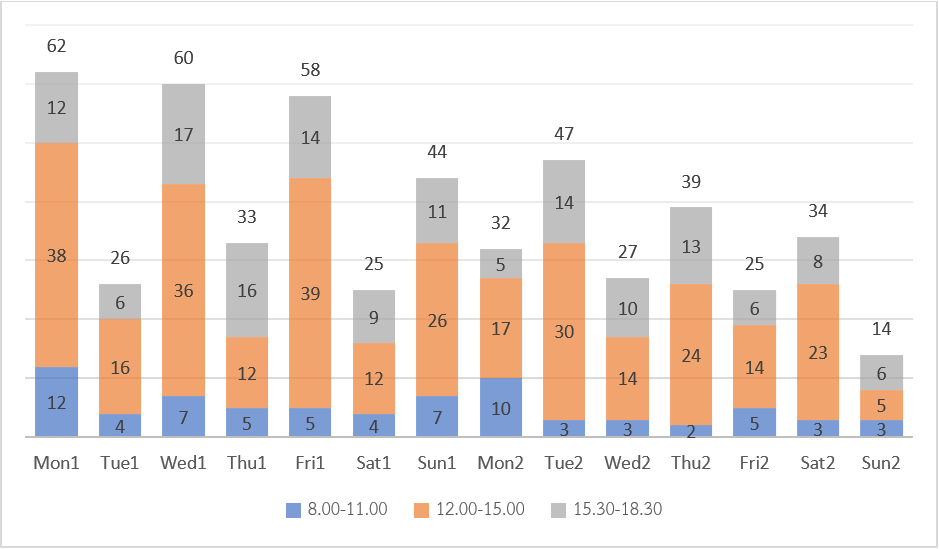
\includegraphics[width=\linewidth]{images/bar_chart_for_final_exam_slot.png}
  \end{center}
  \caption[ความต้องการในการสอบของผู้ตอบแบบสอบถามในแต่ละช่วงเวลาสอบ]{ความต้องการในการสอบของผู้ตอบแบบสอบถามในแต่ละช่วงเวลาสอบ}
  \label{fig:time_slot}     
\end{figure}
\begin{enumerate}
  \item สัปดาห์ที่หนึ่ง เวลา 12.00-15.00น. วันศุกร์ 
  \item สัปดาห์ที่หนึ่ง เวลา 12.00-15.00น. วันจันทร์
  \item สัปดาห์ที่หนึ่ง เวลา 12.00-15.00น. วันพุธ
  \item สัปดาห์ที่สอง เวลา 12.00-15.00น. วันอังคาร
  \item สัปดาห์ที่หนึ่ง เวลา 12.00-15.00น. วันอาทิตย์
  \item สัปดาห์ที่สอง เวลา 12.00-15.00น. วันพฤหัสบดี
  \item สัปดาห์ที่สอง เวลา 12.00-15.00น. วันเสาร์
\end{enumerate}

ซึ่งจากกราฟ \ref{fig:time_slot} ยังสามารถสรุปได้ว่าผู้ทำแบบสอบถามส่วนใหญ่ต้องการที่จะสอบหนึ่งวันเว้นหนึ่งวันเพื่อที่จะได้มีเวลาในการอ่านหนังสือเตรียมสอบสำหรับวิชาในวันถัดไปมากกว่าการสอบติดกัน 
เรายังสามารถบอกเพิ่มเติมได้อีกว่าผู้ทำแบบสอบถามส่วนใหญ่ต้องการสอบในช่วงสัปดาห์แรกของช่วงการสอบมากกว่าช่วงสัปดาห์ที่สองเพื่อที่จะได้มีเวลาพักผ่อนหรือกลับบ้าน หลังจากที่สอบเสร็จแล้ว
\newpage
\subsection{การเก็บข้อมูลตารางสอบ}
หลังจากได้ผลการสำรวจแล้วเราจึงได้ออกสำรวจเพื่อเก็บข้อมูลรายวิชาต่าง ๆ ที่มีการจัดสอบจากแต่ละคณะ โดยได้ทำคำร้องขอข้อมูลไปยังแต่ละคณะ ซึ่งข้อมูลที่ต้องการใช้งาน ได้แก่ ข้อมูลห้องที่สามารถจัดสอบได้พร้อมจำนวนนักศึกษาที่จุได้ในแต่ละห้องของแต่ละคณะ และข้อมูลตารางสอบปลายภาคของแต่ละคณะ เป็นเวลา 6 ปีย้อนหลัง ซึ่งทางเราได้ตั้งสมมติฐานว่าวิชาไหนที่มีการจัดสอบและมีรายชื่อวิชาอยู่ในคำสั่งแต่งตั้งกรรมการคุมสอบของแต่ละคณะนั้น จะมีการจัดสอบปลายภาคจริง ๆ และเวลาที่จัดสอบอยู่ในช่วงเวลาที่สำนักทะเบียนกำหนด

\section{โครงสร้างและการทำงานของโปรแกรม}
\subsection{ข้อมูลที่ต้องใช้ในการจัดตารางสอบ}
ข้อมูลนำเข้าของโปรแกรมจะมีโครงสร้างไดเรกทอรี่และไฟล์ดังที่แสดง

\begin{forest}
  for tree={
    font=\ttfamily,
    grow'=0,
    child anchor=west,
    parent anchor=south,
    anchor=west,
    calign=first,
    inner xsep=7pt,
    edge path={
      \noexpand\path [draw, \forestoption{edge}]
      (!u.south west) +(7.5pt,0) |- (.child anchor) pic {folder} \forestoption{edge label};
    },
    % style for your file node 
    file/.style={edge path={\noexpand\path [draw, \forestoption{edge}]
      (!u.south west) +(7.5pt,0) |- (.child anchor) \forestoption{edge label};},
      inner xsep=2pt,font=\small\ttfamily
                 },
    before typesetting nodes={
      if n=1
        {insert before={[,phantom]}}
        {}
    },
    fit=band,
    before computing xy={l=15pt},
  } 
[root-folder
  [data
    [all-exam-courses
      [all-exam-courses.in,file]
    ]
    [capacity
      [faculty-capacity.in,file]
    ]
    [exam-courses-faculty
      [01.in,file]
      [02.in,file]
      [03.in,file]
      [...,file]
      [19.in,file]
      [20.in,file]
      [21.in,file]
    ]
    [regist
      [regist-academic\_year-semester.in,file]
    ]
    [sched
      [conflicts.in,file]
      [courses.in,file]
    ]
  ]
  [final\_exam\_graph\_coloring.py,file]
]
\end{forest}
\begin{figure}
  \begin{center}
    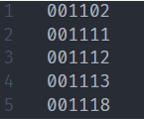
\includegraphics[]{images/all-exam1.png}
  \end{center}
  \caption[ตัวอย่างไฟล์รายวิชาที่มีสอบ]{ตัวอย่างไฟล์รายวิชาที่มีสอบ}
  \label{fig:all_courses}     
\end{figure}
\begin{figure}
  \begin{center}
    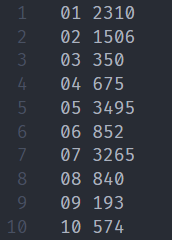
\includegraphics[]{images/capacity1.png}
  \end{center}
  \caption[ตัวอย่างไฟล์ความจุห้องสอบ]{ตัวอย่างไฟล์ความจุห้องสอบ}
  \label{fig:capacity}     
\end{figure}
\begin{figure}
  \begin{center}
    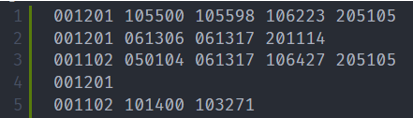
\includegraphics[]{images/regist1.png}
  \end{center}
  \caption[ตัวอย่างไฟล์ลงทะเบียนของนักศึกษา]{ตัวอย่างไฟล์ลงทะเบียนของนักศึกษา}
  \label{fig:regist}     
\end{figure}
\begin{figure}
  \begin{center}
    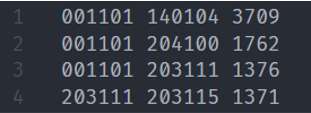
\includegraphics[]{images/conflicts1.png}
  \end{center}
  \caption[ตัวอย่างไฟล์คู่วิชาที่มีนักศึกษาลงทะเบียนพร้อมกัน]{ตัวอย่างไฟล์คู่วิชาที่มีนักศึกษาลงทะเบียนพร้อมกัน}
  \label{fig:conflicts}     
\end{figure}
\begin{figure}
  \begin{center}
    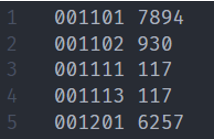
\includegraphics[]{images/courses1.png}
  \end{center}
  \caption[ตัวอย่างไฟล์วิชาที่มีนักศึกษาลงทะเบียน]{ตัวอย่างไฟล์วิชาที่มีนักศึกษาลงทะเบียน}
  \label{fig:courses}     
\end{figure}
\begin{itemize}
  \item ในโฟลเดอร์ all-exam-course ประกอบไปด้วยไฟล์ <all-exam-course.in> จำนวน 1 ไฟล์ ซึ่งเป็นไฟล์ text ในไฟล์แต่ละบรรทัดประกอบด้วยรหัสวิชาที่มีการจัดสอบ หนึ่งบรรทัดต่อหนึ่งรหัสวิชา ดังภาพที่ \ref{fig:all_courses}
  \item ในโฟลเดอร์ capacity ประกอบไปด้วยไฟล์ <faculty-capacity.in> จำนวน 1 ไฟล์ ซึ่งเป็นไฟล์ text ในไฟล์แต่ละบรรทัดประกอบไปด้วย รหัสคณะ และจำนวนความจุรวมของห้องสอบของคณะนั้น ๆ แต่ละส่วนคั่นด้วย เว้นวรรค (space) ดังภาพที่ \ref{fig:capacity}
  \item ในโฟลเดอร์ exam-courses-faculty ประกอบไปด้วยไฟล์ <01.in> ถึง <21.in> ซึ่งเป็นไฟล์ text โดยตั้งชื่อไฟล์ตามรหัสคณะ ในแต่ละไฟล์ประกอบด้วย รหัสวิชาที่มีการจัดสอบ หนึ่งบรรทัดต่อหนึ่งรหัสวิชา ดังภาพที่ \ref{fig:all_courses} 
  \item ในโฟลเดอร์ regist ประกอบไปด้วยไฟล์ <regist-ปีการศึกษา-เทอม.in> ซึ่งเป็นไฟล์ text ในไฟล์ประกอบไปด้วยข้อมูลลงทะเบียนของนักศึกษาแต่ละคน แต่ละบรรทัดประกอบด้วย รหัสวิชาที่นักศึกษาหนึ่งคนลงทะเบียนในเทอมนั้น ๆ แต่ละวิชาคั่นด้วย เว้นวรรค (space) ดังภาพที่ \ref{fig:regist}
  \item ในโฟลเดอร์ sched ประกอบไปด้วยไฟล์ <conflicts.in> ดังภาพที่ \ref{fig:conflicts} และ courses.in ดังภาพที่ \ref{fig:courses} ซึ่งเป็นไฟล์ text ในไฟล์ <conflicts.in> ประกอบด้วย รหัสวิชาสองวิชาที่มีนักศึกษาลงทะเบียนพร้อมกันในภาคการศึกษานั้น ๆ และ จำนวนนักศึกษาที่ลงทะเบียนคู่วิชานี้ แต่ละส่วนคั่นด้วย เว้นวรรค (space) ในไฟล์ courses.in ประกอบด้วยรหัสวิชา และจำนวนนักศึกษาที่ลงทะเบียนในวิชานั้น ๆ แต่ละส่วนคั่นด้วย เว้นวรรค (space)
\end{itemize}

\subsection{รูปแบบของผลลัพธ์จากการจัดตารางสอบ}
ข้อมูลผลลัพธ์ของโปรแกรมจะเป็นไฟล์ csv ที่ระบุรายวิชาคู่กับ slot ที่สอบของรายวิชานั้น ๆ โดยจะมีข้อมูลใช้สำหรับ mapping หมายเลข slot เป็นวันและเวลาสอบ

\subsection{การออกแบบอัลกอลิทึมและแผนผังการทำงานของโปรแกรม}
ในการออกแบบอัลกอริทึมสำหรับใช้ในการจัดตารางสอบ จะใช้วิธีการระบายสีกราฟ (graph coloring) 
โดยจะแปลงรายวิชาที่ต้องจัดสอบเป็นโหนดของกราฟ (node) 
และคู่วิชาที่มีนักศึกษาคนใด ๆ ลงทะเบียนพร้อมกันในเทอมนั้นจะถูกจัดให้สอบพร้อมกันไม่ได้ 
จึงจะถูกแปลงเป็นเส้นเชื่อมในกราฟ (edge) จำนวนนักศึกษาที่ลงทะเบียนในคู่วิชานั้น ๆ จะถูกแปลงเป็น edge weights
และช่วงเวลาที่แต่ละวิชาจัดสอบ (slot) จะถูกแปลงเป็นสีของโหนด
โดยผลรวมของ edge weights ของกราฟเรียกว่า conflict
จำนวนเส้นเชื่อมทั้งหมดที่เข้า-ออก จากกราฟจะเรียกว่า ดีกรี (degree) 
โดยอัลกอริทึมจะมีลำดับการทำงานตามรูปที่ \ref{fig:flowchart} 
โดยเมื่อจะรันโปรแกรมจะต้องเลือกอัลกอริทึม 1 รูปแบบจากทั้งหมด 4 รูปแบบ ดังขั้นตอนที่ 1
และอัลกอริทึมจะมีรูปแบบการทำงานทั้งหมด 4 รูปแบบ โดยแต่ละรูปแบบจะมีความแตกต่างกันที่ลำดับการเลือกโหนดมาเพื่อละบายสี
โดยแต่ละรูปแบบจะมีการเรียงลำดับ ดังนี้

\subsection{รูปแบบของอัลกอลิทึม}
\begin{enumerate}
  \item รูปแบบที่ 1 BFS-DEG ทำ BFS จากแต่ละโหนดโดยมีการเรียงลำดับความสำคัญของโหนดที่จะจัดช่วงเวลาสอบก่อน โดยเรียงจาก
  ดีกรีของโหนด จำนวนนักศึกษาที่ลงทะเบียน จำนวน conflict ของโหนด และหากทุกอย่างเท่ากันจะเรียงตามรหัสวิชา โดยเรียงจากมากไปน้อยตามลำดับ
  เมื่อจัดช่วงเวลาสอบให้ครบทุกโหนดเพื่อนบ้านแล้วจะเริ่มกระบวนการนี้ซ้ำที่โหนดเพื่อนบ้านถัดไป จนกว่าจะจัดช่วงเวลาสอบได้ครบทุกโหนด
  \item รูปแบบที่ 2 DEG จัดช่วงเวลาสอบให้แต่ละโหนดโดยมีการเรียงลำดับความสำคัญของโหนดที่จะจัดช่วงเวลาสอบก่อน โดยเรียงจาก
  ดีกรีของโหนด จำนวนนักศึกษาที่ลงทะเบียน จำนวน conflict ของโหนด และหากทุกอย่างเท่ากันจะเรียงตามรหัสวิชา โดยเรียงจากมากไปน้อยตามลำดับ
  \item รูปแบบที่ 3 BFS-STD ทำ BFS จากแต่ละโหนดโดยมีการเรียงลำดับความสำคัญของโหนดที่จะจัดช่วงเวลาสอบก่อน โดยเรียงจาก
  จำนวนนักศึกษาที่ลงทะเบียน ดีกรีของโหนด จำนวน conflict ของโหนด และหากทุกอย่างเท่ากันจะเรียงตามรหัสวิชา โดยเรียงจากมากไปน้อยตามลำดับ
  เมื่อจัดช่วงเวลาสอบให้ครบทุกโหนดเพื่อนบ้านแล้วจะเริ่มกระบวนการนี้ซ้ำที่โหนดเพื่อนบ้านถัดไป จนกว่าจะจัดช่วงเวลาสอบได้ครบทุกโหนด
  \item รูปแบบที่ 4 STD จัดช่วงเวลาสอบให้แต่ละโหนดโดยมีการเรียงลำดับความสำคัญของโหนดที่จะจัดช่วงเวลาสอบก่อน โดยเรียงจาก
  จำนวนนักศึกษาที่ลงทะเบียน ดีกรีของโหนด จำนวน conflict ของโหนด และหากทุกอย่างเท่ากันจะเรียงตามรหัสวิชา โดยเรียงจากมากไปน้อยตามลำดับ
\end{enumerate}

\begin{figure}
  \begin{center}
    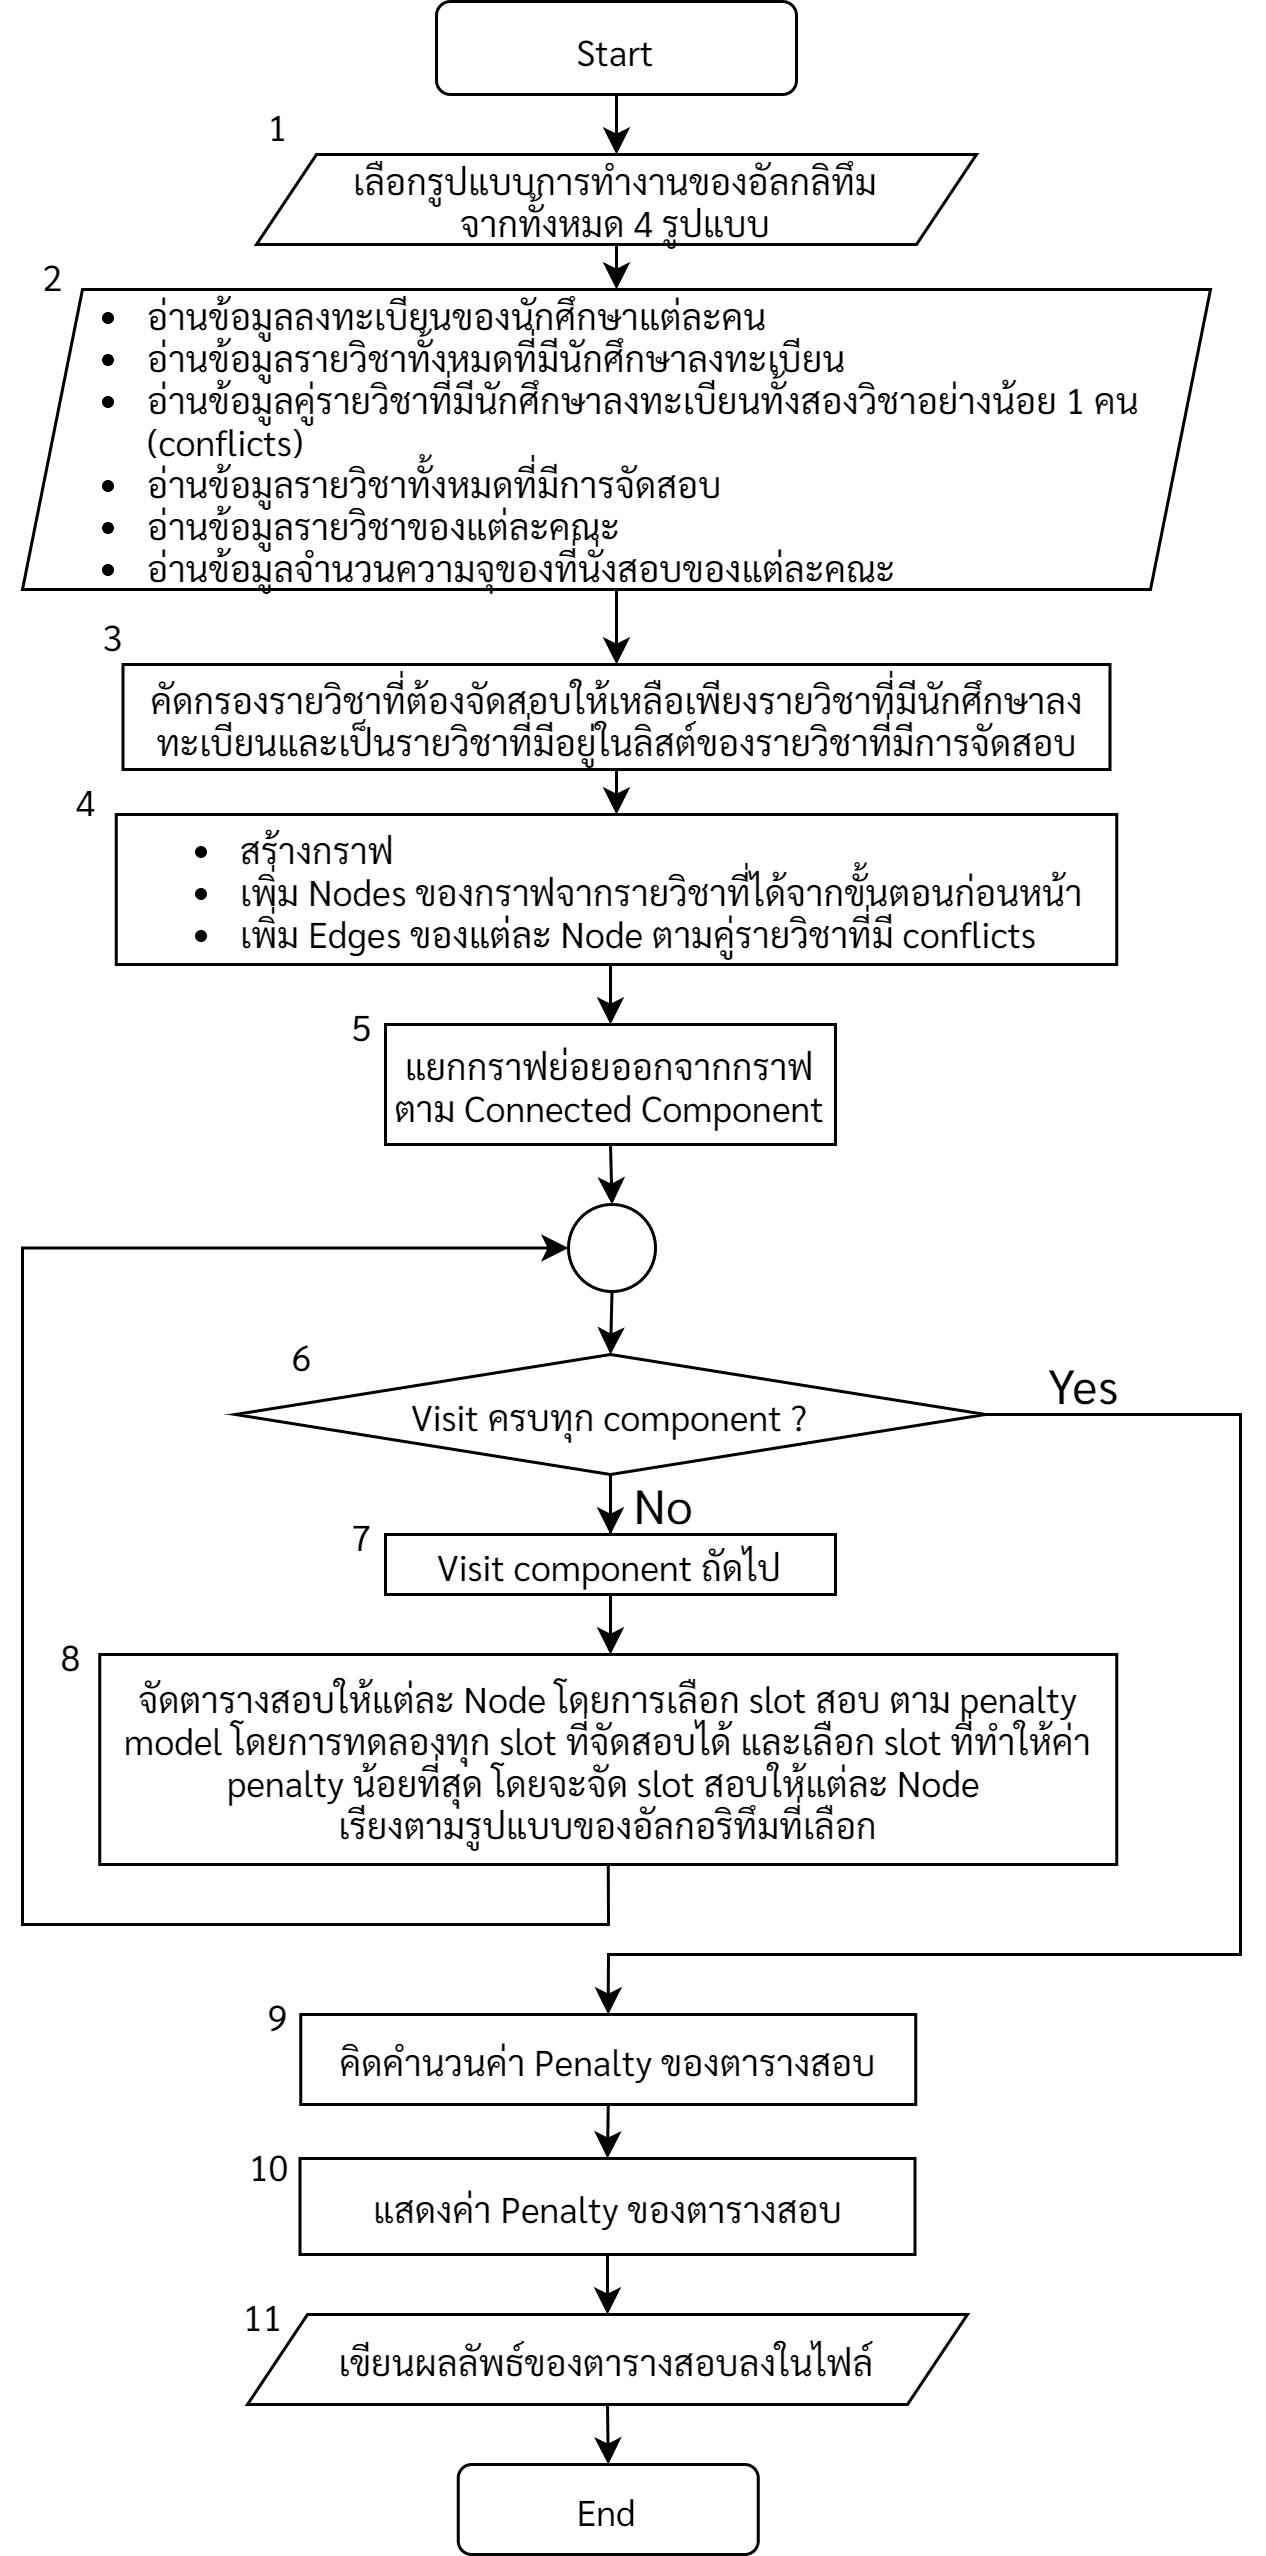
\includegraphics[]{images/exam_sched_flowchart.png}
  \end{center}
  \caption[แผนผังการทำงานของโปรแกรม]{แผนผังการทำงานของโปรแกรม}
  \label{fig:flowchart}     
\end{figure}
